\documentclass[12pt,a4paper,oneside]{scrartcl}
\usepackage[left=2.5cm,right=2.5cm,top=3cm,bottom=3cm]{geometry}

\usepackage[utf8x]{inputenc}
\usepackage[T1]{fontenc}
\usepackage[english]{babel}

\usepackage[fleqn]{mathtools} %Replaces AMSMATH

\usepackage{fancyhdr}

%Nice Tables
\usepackage{tabularx}
\usepackage{booktabs}



%Section Heading font
\setkomafont{section}{\normalfont\large\rmfamily\bfseries}
\setkomafont{subsection}{\normalfont\normalsize\rmfamily\bfseries}
\setkomafont{sectioning}{\normalfont\large\rmfamily\bfseries}

\title{Title}
\author{Name}
\date{Date}


\pagestyle{fancy}
\lhead{\footnotesize Astrophysics SH2402 Seminar - Microlensing \\ date}
\rhead{\footnotesize Linda Eliasson, Alejandro Ruiz \\ Albyn Lowe, Michael Bühlmann}


\begin{document}

\section{Introduction to microlensing}
\subsection{History}
\subsection{Theoretical Background}
In gravitational microlensing, we study what happens to the light from a distance star (the source) when another star (the lens) passes in the field of view, see figure \ref{fig:Microlens_draw}\footnote{www.astro.cornell.edu/academics/courses/astro201/microlensing.htm}. The light from the source creates a so called Einstein ring arounde the lensing star. The ring is clearly seen in figure \ref{fig:EinsteinRing}\footnote{en.wikipedia.org/wiki/Gravitational\_microlensing} from the Hubble telescope.
\begin{figure}[p]
\centering
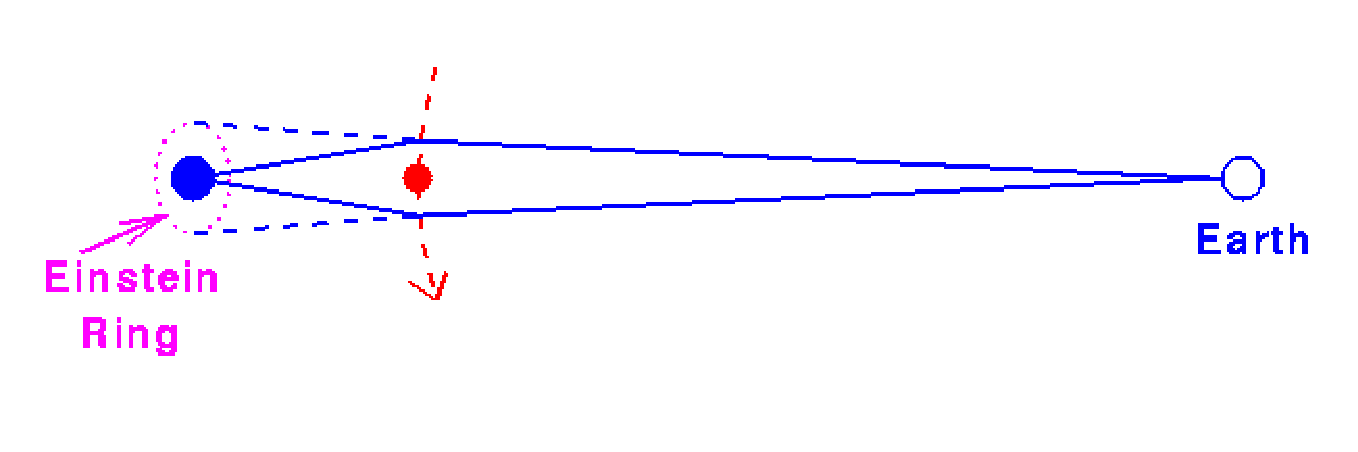
\includegraphics[width=0.7 \textwidth]{microlens_draw}
\caption{\emph{Microlensing event. A star passes between a source star and the observer, causing the source light to bend.}}\label{fig:Microlens_draw}
\end{figure}
\begin{figure}[p]
\centering
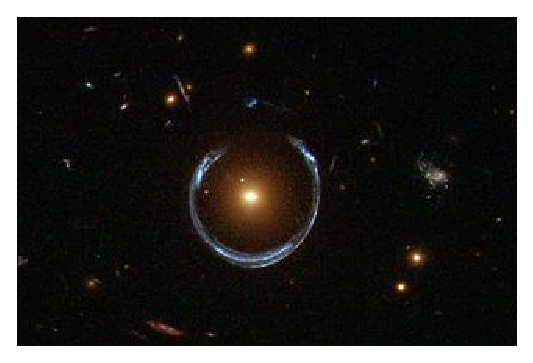
\includegraphics[width=0.3 \textwidth]{Wiki_A_Horseshoe_Einstein_Ring_from_Hubble}
\caption{\emph{An Einstein ring seen from the Hubble telescope.}\label{fig:EinsteinRing}}
\end{figure}

Preferably, the transition should not take more than a couple of weeks or months, so the stars can't be too far apart. So when standing on earth, looking at a microlensing event, it looks like the source star quickly brightens as the lens passes by - the light magnifies, as seen in figure \ref{fig:LightCurve}\footnote{www.perthobservatory.we.gov.au/research.htm}. 


\begin{figure}[p]
\centering
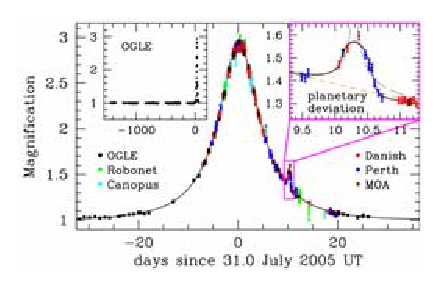
\includegraphics[width=0.5 \textwidth]{LightCurve_OGLE2005BLG390Lb}
\caption{\emph{The light curve from the exoplanet OGLE-2005-BLG-390Lb.}\label{fig:LightCurve}}
\end{figure}



\section{Applications today}

\subsection{Dark Matter}
Observing the rotational speed of galaxies, we can see that there must be more matter than what is visible to us. This unknown part of matter is called dark matter and makes up about 90\% of the matter in the Universe. Observations suggest that the dark matter forms  spherical haloes around the centers of the galaxies.

One theory about dark matter is that it's composed (at least in part) of dim objects with smaller mass than the sun like brown and white dwarfs and black holes. Those objects are called MACHOS (massive compact halo objects). Since the 90ties there have been approches to find such objects using microlensing. Astronomers indeed detected MACHOs in this way, but not nearly enough to explain the mystery. MACHOs account at most up to 20\% of the dark matter halo.

\subsection{Exoplanets}
If there is only one lens, the light magnification is symmetrical. If the lensing star has planets orbiting around it, the magnification will not be symmetrical since also the planets will bend the light from the source - they too will act as lenses. The light magnification will therefore look something like the zoomed part in figure \ref{fig:LightCurve}. This figure shows the light curve from the exoplanet OGLE-2005-BLG-390Lb, which has a mass of around $5.5M_{\odot}$

Even with smaller planets orbiting, such as these with the size of the earth, the magnification can get strong enough to see. This makes microlensing a very good tool to detect smaller exoplanets. Another advantage is that it is possible to see planets orbiting very close to the star. However, these microlensing events are quite rare since the stars has to be close enough to each other. It is very easy to miss the light magnification that the transit gives. Then you also miss the opportunity to see if there was a planet there.  



\section{Teaching plans}


\end{document}
